\documentclass{article}
\usepackage{graphicx}
\usepackage{threeparttable}
\usepackage{amssymb}
\usepackage{hyperref}

\usepackage{pdflscape}

\title{Concepts of function in biology and biomedicine}

\begin{document}
\maketitle

\section{Abstract}
\label{sec:abstract}

Several philosophical accounts of disease are constructed at least partly around an objective biological criterion. Under these accounts, we can define disease as the failure of physiological parts or processes to perform their proper function or an ``impairment of normal functioning''. Determining whether a phenotype—such as obesity—is a disease or determining the level of functioning at which some aspect of physiology—such as response to insulin—becomes pathological throws considerable weight on the concept of biological function. However, there are a number of philosophical theories of function, each of which defines function differently. It is not clear which theory—or combination of theories—we should use to explicate the medical conception of function. One reason for this is that we have no systematic way to determine how biologists and medical practitioners conceive of, or write about, function in their respective disciplines. To further complicate matters, natural language is replete with ambiguities, and scientific manuscripts often use technical terms imprecisely. Without a descriptive understanding of how different conceptions of function are used in biology and medicine, we have little hope of bringing insights on biological function to bear on disputes about function and malfunction in medicine. Here we develop a systematic method for analysing biological function by outlining a classification scheme that combines syntactic and semantic analysis in a dependency-grammar framework.

\section{Introduction}
\label{sec:introduction}

Much of philosophy of medicine is concerned with defining issues surrounding the concept of disease.
Philosophical approaches to categorising disease can be broadly divided into two camps: a constructivist view that prioritises social value judgements and a naturalist view that prioritises biological theory.
The former contends that disease should be primarily based on whether society disvalues the condition in question, whereas the latter holds that our categorisation of disease should be primarily based on whether ``something has gone wrong'' in a biological system.
But what does it mean for ``something to go wrong'' with a biological system according to the naturalist view?

Before determining what it means for ``something to go wrong'', one requires a normative framework that can be used to determine what a biological component (trait) ought to do.
To ground their normative claims in biology, many naturalist accounts defer to the notion of function.
If a trait's function is what the trait ought to do, then a dysfunctional trait no longer does what the trait ought to do.
We call this dysfunctional state ``disease''.
But herein lies several problems.
Function is a word with multiple senses in both its colloquial and discipline-specific uses.
Within the discipline of philosophy, there are many theories of biological function, each differing in their claims to normativity (and some with arguably no normative claims whatsoever).
In more applied disciplines, such as biology, medical research, and clinical medicine, it can be unclear which concept of function is being employed or how well usage maps onto philosphical conceptions of function.
% One cannot easily make progress on a theory without first setting a solid foundation.

Experimental philosophy relies, in large part, on extracting meaning from natural language.
If we hope to use experimental philosophy to understand a naturalistic account of disease and dysfunction, we must first clarify how the concept of function (and dysfunction) is used in natural language.
%It is thus crucial that philosophers have methods for identifying which sense of function is used in natural language.
One must solve two broad problems in order to consistently disambiguate real-world usage of biological function (or any word that refers to multiple concepts).
First, one must develop a classification scheme comprising a set of categories, each of which defines a sense (or concept) of function.
The categories within the set should be exhaustive, covering all possible real-world uses of function.
Furthermore, the categories should either be exclusive (i.e. each use of function has one and only one sense) or there should be explicit rules for how one is to deal with membership in overlapping categories (e.g. a hierarchy of definitions or allowing of multiple senses for a single usage). 
Second, one must develop a system that can consistently assign a piece of natural language on biological function (sentence, paragraph, etc.) into its correct category.

The problem of developing a set of categories will typically employ some form of conceptual analysis (and/or leverage earlier conceptual analysis).
We cannot, however, simply paste together existing concepts of biological function.
For one, this will not necessarily generate a set of function concepts that are exhaustive or exclusive.\footnote{For an example with respect to exclusivity, consider that some philosophical concepts of function have closely overlapping features. Say we have two overlapping concepts, such as the causal role and organisational theories of function. We must make some hard decisions when deciding how to incorporate these concepts into a coherent classification scheme. We could choose one category and remove the other, allow both but give one hierarchical precedence over the other when ambiguities arise, allow a single usage to be assigned to both categories, or create a general category that encompasses both concepts. (Here we have chosen the latter approach.)}
Moreover, real-world usage of function does not always align with philosophical concepts of function.
A classification scheme for experimental philosophy will thus necessarily be an amalgamation of philosophical conceptual analysis and discipline-specific usage.

A study has recently attempted this for biological function in the context of de novo gene emergence (cite elife).
The authors chose six categories for their classification scheme: Evolutionary Implications, Physiological Implications, Interactions, Capacities, Expression, and Vague.
The authors started broadly with the two most well-known philosophical concepts of function: causal role and selected effects.
From this base, they iterated through a small dataset of 42 examples (from 20 abstracts), adding categories and refining the scheme as they encountered new usages that did not fit into the existing scheme.
They achieve an exhaustive scheme by implementing a catch-all category of Vague for usage unable to be categorised in one of the other five categories.
They did not require that these categories be mutually exclusive, instead allowing a single usage to have membership in multiple categories.
To categorise each usage of function using the scheme, the authors started by independently reading a paper's title and abstract.
Next they used a list of definitions to assign at least one meaning of function to the example, which were supplemented by a few general coding rules to guide application of the definitions.
One of the most striking fundings from this study was the difficulty of obtaining agreement between the different raters: in only 12\% of cases did all four raters independently assign an example the same category!
After conferring with one another and employing a consensus-based approach, the raters were still only able to assign 62\% of cases to a single category.
Despite having a comprehensive and well-reasoned classification scheme in hand, these authors were not able to consistently categorise real-world usages of function into a single category.\footnote{We had a simlar experience in the course of developing our scheme. Early-on, we used an approach similar to Keeling et. al. (2019) in which we would individually rate sentences, and if there was a disagreement, we would try to categorise the example using a consensus-based approach. (The purpose of this was to identify a set of gold-standard examples that we could use to test the performance of our scheme on.) We frequently disagreed about how to classify certain examples, both independently and through trying to establish consensus.}
This is clearly an immensely difficult problem to solve, and there are likely a number of factors that contributed to the difficulty in unambiguously assigning usages of function to a single concept.
We suggest, however, that a crucial factor lies in the different ways that individual investigators analyse natural language in order to extract meaning.
Without a detailed and standardised framework, the semantic mapping from natural language to a definition of function is bound to inconsistent among different investigators.

In this manuscript, we ask a similar question to Keeling et. al. (2019) but adopt a different methodology.
Our classification scheme does not try to semantically map directly from natural language to definitions of function.
To assign an example to a definition, one instead follows a step-by-step flowchart, answering questions and identifying important features related to function that are contained within a piece of natural language.
We unpack each piece of natural language into one of several common forms.
For example, to be classified as Biological Role (see section ``Senses of function''), an investigator must be able to identify each variable in the unpacked form of ``The function of \emph{ITEM} is \emph{EFFECT} in \emph{SYSTEM}''(e.g. \emph{ITEM} could be ``The heart'', \emph{EFFECT} could be ``to pump blood through'', and \emph{SYSTEM} could be ``the circulatory system'').
By simplifying natural language into simple, common forms, our approach avoids obfuscation of meaning due to variation in syntactic construction and helps standardise the technique for extracting meaning.
Moreover, we provide detailed instructions for how to use the dependency grammar framework and modern natural language processing techniques as aids in identifying the variables in the common forms.

\section{Classification flowchart}
\label{sec:class-scheme}

Our approach was to analyse real-world uses of biological function extracted from scientific papers.
Through an iterative process, we altered our method each time that we encountered common occurences, or general patterns, that our method handled poorly\footnote{will need to expand on this to talk about what we mean by ``poorly'', how we began with consensus, and so forth. Not sure whether all of the general method should be here or whether some of it can go later. Currently pasting the various snippets of text about it in this section}.
Since our focus was on how function is used in biology, we used examples from a wide variety of biological subfields.
Specifically, we used the ARC FoR, matched with WoS/JIF, chose 1 paper from each of the top 5 journals by JIF, giving us xxx examples...(FILL IN LATER)

To begin with, three of the authors (JRC, ZW, SG) independently analysed a subset of the sentences (using definitions and a simple set of classification guidelines, much like Keeling et. al. (2019)).
We then compared our responses, and if our classifications differed, we used a consensus-based approach to categorise examples.

From these examples, we developed a set of ``gold-standard'' examples that we agreed upon, which we were able to use for the purposes of testing our flowchart.

From here, we jointly developed the classification scheme and our pipeline for the analysis of natural language.

Note that there's really 3 layers here: (i) classification scheme (i.e. categories and definitions); (ii) general flowchart; (iii) natural language processing, as an aid to ii.
Actually, probably better to frame it as a new approach towards the classification scheme---we aren't operating on traditional definitions, rather our definitions require that we satisfy certain criteria wrt extracting certain features from a text and placing them in a common structure.

\subsection{Senses of function}
\label{sec:senses-function}

First, we must choose the categories of our classification scheme.\footnote{The Keeling et. al. study was published mid-way through this study, but after we had already developed our categories, and thus differences in the classification schemes reflect the diversity expected when research groups independently tackle similar questions but with different perspectives and focus.}
We decided to use the scheme of Wouters (2003) as our starting point.
Wouters breaks down function into four categories: (i) Biological Activity; (ii) Biological Role; (iii) Biological Advantage; and (iv) Selected Effect.
In Wouters's scheme, Biological Activity is ``what an item does or is capable of doing'', Biological Role describes ``how a certain item or activity contributes to the emergence of a complex capacity of an organism'', Biological Advantage refers to the ``biological value (utility) of a certain trait in comparison with another'', and Selected Effect is ``used in a historical sense to refer to the effects for which a certain trait was selected in the past''.

From this base, we analysed real-world usages of biological function to develop a more comprehensive classification scheme using an iterative process.
We added a new category of function whenever we encountered instances of usage that reoccurred multiple times and could not be classified in one of our existing categories.
To Biological Activity, Biological Role, Biological Advantage, and Selected Effect, we added the following categories: Colloquial, Technical, and Performing.
In some instances, it is not possible to unpack a sentence into a common form and identify the variables.
We thus added the following additional categories whose purpose is to specify what feature was ``missing'' from the sentence: \emph{ITEM} Unspecified, Meaning Unknown: \emph{EFFECT} Unspecified, and Meaning Unknown: \emph{EFFECT} Specified.

\begin{figure}[ht]
  \centering
  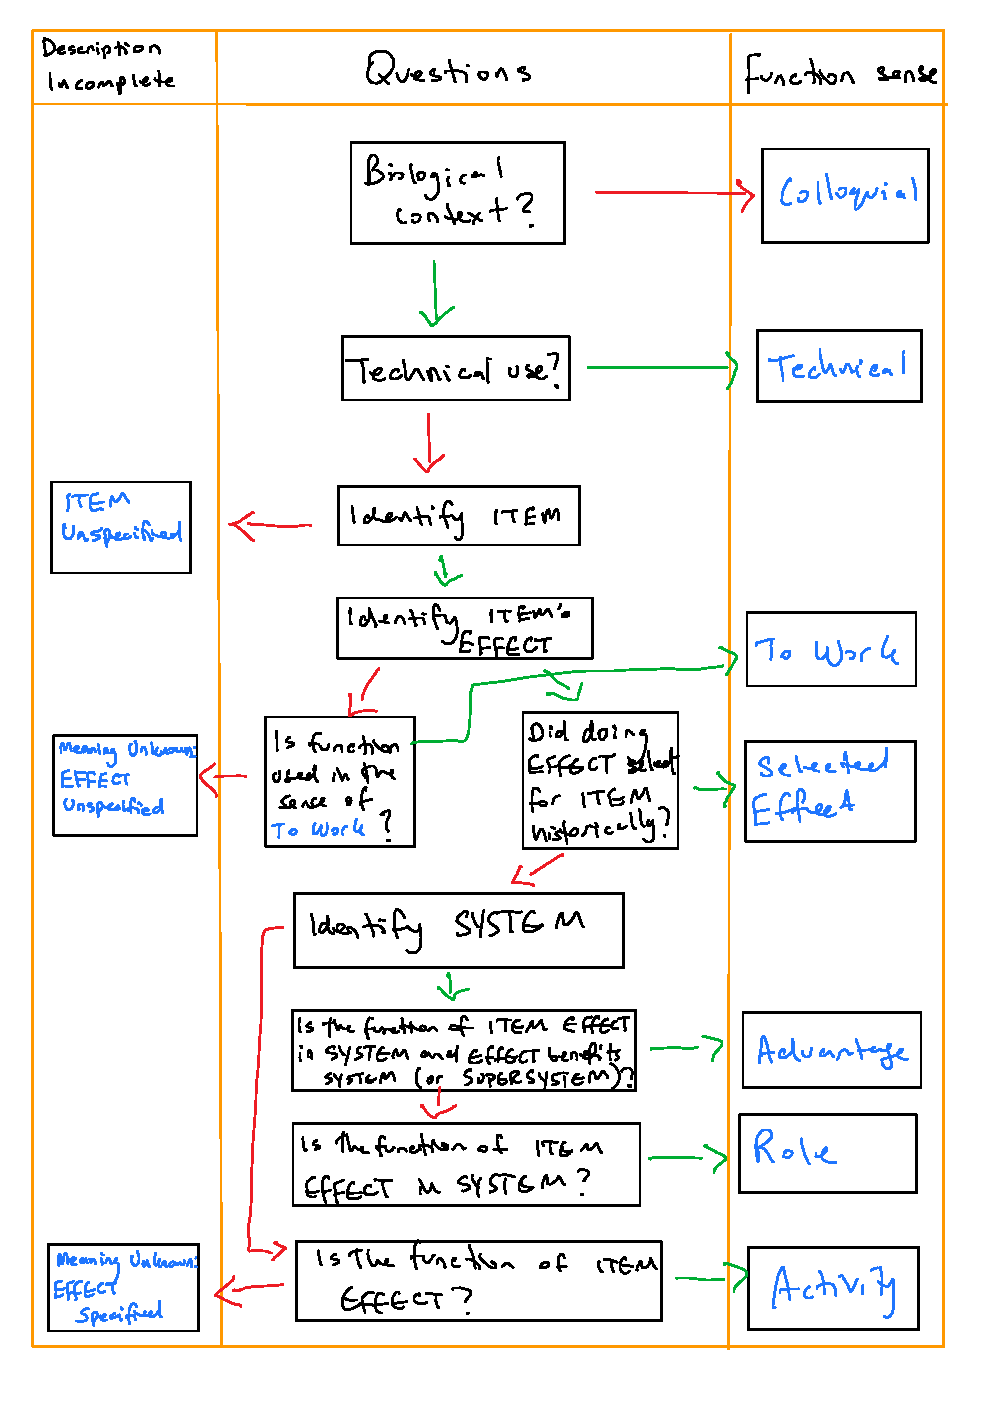
\includegraphics[width=\linewidth]{GeneralFlowchart.pdf}
  \caption[\textbf{Decision flowchart for identifying sense of function.}]{}
  \label{flowchart}
\end{figure}


\begin{landscape}
  \begin{table}
    \small
    \caption{Description of each decision point in the classification flowchart (Figure \ref{flowchart})}
  \begin{tabular}{|p{0.17\linewidth}|p{0.97\linewidth}|}
    \hline
    Decision point & Description \\
    \hline
    Biological context? & Are we dealing with a case of biological function or colloquial use (see \href{http://wordnetweb.princeton.edu/perl/webwn?s=function&sub=Search+WordNet&o2=&o0=1&o8=1&o1=1&o7=&o5=&o9=&o6=&o3=&o4=&h=}{WordNet 3.1} for colloquial definitions)? These examples are rare if one restricts the corpus to scientific papers in biology. Notable exceptions are mathematical functions and programming functions, which we place within Colloquial to simplify the flowchart. \\
    \hline
    Technical use? & Compound phrases such as ``functional ecology'', ``functional biology'', ``functional connectivity'', and so on. These phrases will be familiar to practitioners within a field. Their meanings are multi-faceted and influenced by a field's development and cannot be meaningfully unpacked using a flowchart.  These phrases will often appear multiple times in a manuscript. \\
    \hline
    Identify \emph{ITEM} &  An \emph{ITEM} is something that can be a character or trait of a Darwinian individual. Obvious candidates are concrete nouns, which refer to a physical item (e.g. heart), but it also includes abstract nouns if they refer to a concrete concept (e.g. ``gene'' as used in population genetics, ``boldness'' as a behavioural phenotype, etc.). Importantly, there must be a dependency between function and the \emph{ITEM}---it is not sufficient that a suitable \emph{ITEM} simply appear in the sentence (e.g. ``protein'' is the \emph{ITEM} in  ``protein function aids muscle development'' but ``muscle'' is the \emph{ITEM} in ``protein aids in muscle function''). \\
%    For example, ``gene'' can refer to the concept of an atomic unit of DNA with a well-defined phenotype. This is sufficiently concrete to qualify as a character despite not necessarily mapping onto a physical piece of DNA. 
    \hline
    Identify \emph{ITEM}'s \emph{EFFECT} & \emph{EFFECT} is what the \emph{ITEM} does (or, less commonly, has done to it). \emph{EFFECT} is a verb or verb phrase, but it might not always act as a verb in the text, so long as it can be turned into a verb through word conversion (e.g. ``contribute to transcription'' could be converted to the verb ``transcribe''). \\
    \hline
    Is function used in the sense of Perform? & A heuristic is whether you can substitute ``\emph{ITEM} function'' (or equivalent, depending on the sentence) with ``how well \emph{ITEM} performs'', ``a working \emph{ITEM}'', or similar into the raw sentence without loss of meaning. For example, ``Liver function is important for health'' might become ``A working liver is important for health'' without loss of meaning.\\
    \hline
    Did doing \emph{EFFECT} select for \emph{ITEM} historically? & Can it fit the following form: the function of \emph{ITEM} is to \emph{EFFECT} such that doing \emph{EFFECT} in the past caused \emph{ITEM} to be selected or maintained in a population (relative to an actual or counterfactual historical alternative to \emph{ITEM})? An example would be ``zebra stripes evolved to reduce insect bites'' as reducing insect bites (\emph{EFFECT}) has selected for zebra stripes (\emph{ITEM}).\\
    \hline
    Identify \emph{SYSTEM} & A \emph{SYSTEM} is either a Darwinian individual, or a complex system within an individual, that contains the \emph{ITEM}. The \emph{EFFECT} of the \emph{ITEM} on the \emph{SYSTEM} contributes to a capacity of the \emph{SYSTEM}. As a heuristic for identifying the \emph{SYSTEM}, you can ask  ``how does \emph{ITEM} produce \emph{EFFECT}?'' or ``for what is \emph{ITEM} producing \emph{EFFECT} used?''. \\
    \hline
    Is the function of \emph{ITEM} \emph{EFFECT} in \emph{SYSTEM} and \emph{EFFECT} benefits \emph{SYSTEM} (or \emph{SUPERSYSTEM})? & Consider ``Transcript X functions to regulate expression in the liver, which improves liver performance through regulation of glycogen storage.''. We can unpack this as ``The function of \emph{TRANSCRIPT X} is to \emph{REGULATE EXPRESSION} in \emph{GLYCOGEN STORAGE IN THE LIVER} and \emph{REGULATING EXPRESSION} benefits [improves performance of] \emph{THE LIVER}''. Note the statement's contrastive nature: ``improves liver performance'' indicates that transcript X is being compared to an (unstated) alternative (e.g. transcript Y). Although contrast will often occur, it is not required. For example, we would still classify this example as Biological Advantage if we replaced ``improves liver performance'' with ``aids metabolic control''. Although this alteration removes the contrast, it nevertheless describes a benefit to a supersystem (metabolic system). (A \emph{SUPERSYSTEM} is a system that contains \emph{SYSTEM}.) \\
    \hline
    Is the function of \emph{ITEM} \emph{EFFECT} in \emph{SYSTEM}? &  Biological Role is not contrastive, and it does not contain language indicating a benefit to a system (or supersystem). An example is ``Transcript X functions to regulate expression in the liver, which plays a role in regulation of glycogen storage''. This statement neither contrasts transcript X with an alternative---it simply describes how transcript X contributes to a capacity of the \emph{SYSTEM}---nor explicitly describes a benefit to the \emph{SYSTEM}.  \\
    \hline
    Is the function of \emph{ITEM} \emph{EFFECT}? &  Biological Activity is Biological Role when no \emph{SYSTEM} is specified. An example is ``Transcript X functions to regulate expression'', which simply describes what transcript X does. We do not know how (or in what system) it is being used. \\
    \hline
  \end{tabular}
\end{table}
\end{landscape}

\subsection{Relation between Biological Activity, Role, and Advantage}\footnote{need to improve organisation of these section and the previous, as there's some overlap/redundancy}
\label{sec:relat-betw-funct}

The categories of Biological Activity, Biological Role, and Biological Advantage are conceptually related.
The relationship between Biological Activity and Role is straightforward: a Biological Role is a Biological Activity that contributes to the capacity of a organism (or, more generally, to the capacity of a system). 
The difference between Biological Role and Biological Advantage is summed up, in Wouters's words, by ``a distinction between 'how it is used' (role) and 'how it is useful' (advantage)'' (wouters2003).
We can thus think of Biological Advantage as a Biological Role that benefits an organism by virtue of contributing to a capacity of a system (of that organism).

We classify these three categories in a hierarchical manner, such that Advantage $>$ Role $>$ Activity.
By this we mean that if an example is classified as Biological Advantage, it has also satisfied the criteria for Role and Activity, and if classfied as Role, then it has also satisfied the criteria for Activity.
There are three benefits behind our approach: (i) it neatly captures the relation between these categories within the context of our classification process, as each category is associated with identifying additional feature(s) (\emph{ITEM} and \emph{EFFECT} for the base category of Biological Activity, \emph{SYSTEM} for Biological Role, and a benefit of \emph{EFFECT} toward \emph{SYSTEM} (or \emph{SUPERSYSTEM}) for Biological Advantage); (ii) it is an effective method for developing a classification with mutually-exclusive categories (there would be significant overlap without a hierarchical system, e.g. every Biological Role would also be a Biological Activity); (iii) it allows for categories to be easily combined \emph{post hoc} if desired (see next section for an example)

\subsubsection{Biological Activity}
\label{sec:biological-activity-1}

Biological Activity answers the question ``what does it do?''.
It was first(?) described by Neander (1995), which she called ``minimal function''.
It deals with biological characters (e.g. a biological item, feature, or behaviour), describing what these characters do (or are capable of doing) (Wouters2003).
It has received relatively little philosophical attention, likely because a statement of Biological Activity leaves out important information about how the character is used or why it exists.
Indeed, Biological Activity is often ignored or subsumed under Biological Role, with the resulting category typically being termed ``causal role'' function after Cummins (1975).
We have chosen to keep this distinction for two main reasons.
We believe that Biological Activity does reflect some actual biological use, most notably in the infamous ENCODE study whose goal was to map functionality across the human genome (encode2012).\footnote{It is commonly stated that ENCODE used a causal role definition (e.g. cite1, cite2), but we believe this to be a conflation of Biological Activity and Biological Role. ENCODE focused on correlates of biological activity (encoding protein or non-coding RNA, or displaying a biological signature such as protein binding or a specific chromatin structure) without trying to establish how this activity is used to generate a complex capacity in the wider system.}
Second, keeping the distinction preserves information.
If an investigator believes that the distinction between Biological Activity and Role is spurious, then they can always combine (labelled examples of) the two categories into a single category during the analysis phase.
But one cannot separate these categories \emph{post hoc} if they were originally classified as a single category.

\subsubsection{Biological Role}
\label{sec:biological-role}

Biological Role answers the question ``how is it used?''.
It is closely linked to causal role or mechanistic theories of function (e.g. Cummins 1975, Wouters also cites Bechtel/ Richardson 1993 and Craver 2001).
Like Activity, it deals with biological characters (wouters2003), describing how a character's effect can contribute to a capacity of a complex system.
In addition to causal theories, some real-world uses of organisational theories of function (mossio2009) will likely fall under Biological Role.
Organisational theories differ from causal theories in that they use the notion of a closed and differentiated self-maintaining organisation as a basis for teleology and normativity.
But organisational theories might be classified as Biological Role if the self-maintenance aspect is omitted or downplayed in a particular usage.

\subsubsection{Biological Advantage}
\label{sec:biological-advantage}

Biological Advantage answers the question ``how does it help?''.
It is closely linked with [see garson2016, who calls it fitness-contribution, for some different theories under this broad umbrella; mossoi2009 also mentions Bigelow and Pargetter [1987]; Canfield [1964]; Ruse [1971]].
In Wouters's characterisation, Biological Advantage deals with traits (specific variants of a character), and it is contrastive in nature, describing how a trait's effect has benefits relative to an alternative trait.
Wouters's interpretation of advantage is somewhat more general than the aforementioned theories that focus explicitly on fitness benefits for Darwinian individuals.
Wouters's definition requires that an \emph{ITEM} demonstrate biological value (or utility) over an alternative.
While Wouters states that the ultimate benchmark for biological value is fitness, he acknowledges that Biological Advantage statements may simply describe ``the efficiency with which a certain biological role is performed''.
In these sorts of statements, there is an implicit assumption that improved efficiency of this role benefits the individual, and that it does so in such a way that it correlates with fitness.
This approach will thus include false-positives in cases where the benefits identified correlate poorly with fitness.
In practice, this means that the Wouters's characterisation of Biological Advantage is quite permissive, being satisfied if an organism can do \emph{EFFECT} better with \emph{ITEM} than with an alternative trait.

Some have argued, in opposition to Wouters, that Biological Advantage need not be contrastive (or be limited to dealing with traits), instead focusing on how it contributes to survival (garson2016 referencing buller1998).
There are obvious parallels between a non-contrastive view of Biological Advantage and organisational theories of function, which focus on how an \emph{ITEM}'s \emph{EFFECT} contributes to self-maintenance [a non-contrastive benefit] of a \emph{SYSTEM}.
With this in mind, we take a very general view of Biological Advantage, adopting Wouters's permissive interpretation of biological advantage as improving a biological role's efficiency without requiring that the characterisation be contrastive.\footnote{We also found that a strict philosophical interpretation of Biological Advantage meant that it could be difficult to identify all the requisite components within a sentence, leading to few examples being characterised as Biological Advantage.}
For our purposes, any explicit mention of a benefit to a system of a Darwinian individual is sufficient for an example to be categorised as Biological Advantage instead of Biological Role.
Usages of organisational theories explicitly mentioning the benefits of self-maintenance will thus fall under Biological Advantage (as mentioned previously, those usages of organisational theories that omit explicit references to the benefits of self-maintenance will likely fall under Biological Role).

\subsection{Function as Work}
\label{sec:funct-as-perf}

We identify another common use of function, namely that of Work.
This use has an analog in one of the colloquial senses of function, namely ``to work as expected''.
An example of this usage is ``liver function is important for human health''.
Here function does not refer to a function of the liver (e.g. ``the liver functions to store glycogen''), but rather it refers to the \emph{functioning} of the liver.
We could express the same meaning in ``liver function is important for human health'' with ``a working liver is important for human health'' or with ``liver dysfunction harms human health''.
The former illustrates the sense in which function is being used, while the latter highlights the normative component of this sense of function.

Indeed, for an item to ``work as expected'' implies that we have a normative basis for believing how the item ought to function.
The normative basis might derive from a philosophical theory (e.g. selected effects or the organisational theory), but it might equally have a poorly-justified basis.
Consider a statement such as ``The gene is transcribed and thus is functional''.
What is the normative basis behind this statement?
It appears to adopt some form of a Biological Activity definition, namely that for function it is sufficient that a gene (item) is transcribed (effect) without regard for how it is used within a system.
There might be an explicit set of criteria behind this definition---as in the ENCODE project---but it could also be the case that the author simply has a vague notion that a gene that does anything is functional (i.e. the complement to the notion that a non-functional gene is one that does nothing).
For this category, the important thing is whether a normative basis exists---we areare agnostic as to how the normative basis is constructed (as this can be impossible to determine in a short piece of natural language).

This use of function differs from Activity, Role, and Advantage, which are all ``type'' level designations (dealing with characters or traits) in that it focuses on token level designations.
Function as Work is concerned with how an item has developed in a particular individual (or possibly group of individuals in the case of a syndrome)

old stuff below

 Although it must be said that this isn't the cleanest distinction. While we'll want to ascribe a dysfunctional state (e.g. disease) to an individual, we might cluster underlying etiologies into a single coarse grain phenotype (e.g. a syndrome). Might also cluster a single genotype change (e.g. mito diseases). This could also be without regard for trait (e.g. some mito diseases will apply to the character (all human mito haplotypes), though need to check that this is true), but perhaps some are specific to some traits.
Note that I think part of this comes down to the fact that it's not well-defined whether a new token is a new trait or whether it is a dysfunctional member of the type (i.e. are we dealing with a collection of dysfunctional tokens who are grouped based on either a common inheritance, common architecture, common phenotype, or a new trait type? (you could go via inheritance vs ontogeny but there might be some diseases that are hard to tease apart here? e.g. mito disease could be a mutation from mother, stable inheritance, mutation in zygote, etc.---would we really distinguish them if they're the same structurally? I need to be careful here because I'm claiming that dysfunction is ontogenic so I really need to be able to make the claim that dysfunction is token-level which means syndromes/diseases are collections of token dysfunctions. Note Neander 2017 says that malfunctions are token level.)
One way of talking about when a dysfunction becomes a trait is when it is heritable...this will lead to some odd cases (mitochondrial diseases becoming traits), or we just accept that harmful dysfunctions that are heritable are a grey zone. Huntington's disease is another good example because it can be caused by ``slippage'' of genetic repeats so is ontogenic in this sense, yet it is also heritable.
Neander (2017) actually seems to want to say that ``not performing function = malfunction'' due to mismatch (pg 1152)

Will also need to address organizational theories and their claim of normativity. Will need to sidestep all the details but basically the main point is for dysfunction you need two things: (i) a Cummins-style functional analysis but of how an item is working in a token (not character); and (ii) a normative grounding that tells you how it ``ought to work''. All approaches must borrow elements from each other to make this work (SE needs CR; CR needs SE or some other framework that ascribes type-level normativity; organizational must borrow elements from CR and SE (for the latter need to see whether they've developed the reproduction aspect). So the point is that we need pluralism of the three function questions to get at dysfunction.

We have a different approach with regard to how we deal with potential overlap between categories.
While Keeling et. al. (2019), allowed a single usage of function to have multiple senses, our usages of function have a single sense (i.e. our sense categories are mutually exclusive).

\section{Analysis of natural language}
\label{sec:analys-natur-lang}

Function has many derivatives (e.g. functional) and can be used in different parts of speech (noun, verb, etc.), which significantly complicates analysis of natural language.
If we focus just on the forms of function when used as a noun, we have the singular ``function'' (``the function of the heart''), and the plural ``functions'' (``the heart has many functions''), and the derivative ``functionality'' (``the functionality of the heart'').
Grammatical relations also vary.
In ``the function of the heart'' and ``the functionality of the heart'', function is the subject, whereas for ``the heart has many functions'', function is the direct object.
Aside from its use as a noun, ``functions'' (and ``function'') can also be used as a verb (``the heart functions to pump blood'').
We also encounter cases such as the gerund form ``functioning'', which is the -ing form of the verb ``function'' that acts as a noun (``functioning is important for hearts'')!
And to complicate matters even further, ``functioning'' might be a present participle instead of a gerund, in which case it either acts as an adjective (``the functioning heart'') or to form verb tense (``the heart was functioning''). Suffice it to say, when dealing with real-world sentences, the sheer variety of syntactical forms present a challenge for semantic interpretation of function.
Thus, the first component of our approach is to simplify these diverse syntactic constructions into common forms.
For example, a simple common form would be ``The function of \emph{x} is to \emph{y}'', where \emph{x} is a biological item (e.g. ``heart'') and \emph{y} indicates what the biological item does (e.g. ``pump blood'').

To simplify comparison of syntactically-diverse constructions, we will use word conversion to convert from derivations of "function" to its root form function (specifically morphological derivation and inflection). We will use morphological derivation to convert between parts of speech (e.g. adjective -> noun) and inflection to convert between number, tense and aspect (e.g. the plural functions to function). The key consideration during conversion is that we maintain (and convert if necessary) the dependencies between "function" and other parts of the sentence. What I will describe here is a method for converting these derivations of the word function to its base form (the verb or noun "function"), while at the same time, keeping track of and converting the form (where necessary) of the dependencies of "function". The idea is to rework the sentence such that semantic relations can be cast into a standard form.

\section{advice for best practices}
\label{sec:advice-best-pract}

should also mention that the elife paper has poor inter-observer agreement even though it overfits its definitions by testing on the ``train set''.

add some stuff on automation here and how some steps are better suited to statistical inference rather than rules (e.g. for selected effects and biological advantage it might be easier to label a bunch of examples and train a transformer model using supervision to classify the examples than it would be to provide bullet-proof rules)

Actually this section is probably unnecessary, likely too technical

\section{example sentences}
\label{sec:example-sentences}

test=nlp("In general, these transcripts show little evidence of purifying selection, suggesting that many of them are not functional")

effect unspecified (Question: what have these transcripts done to cause them to be selected? Answer: we don't know, it's not specified)

change to

test=nlp("In general, these transcripts show evidence of translation into proteins, suggesting that many of them are functional")

either activity or role

change to

test=nlp("In general, these transcripts show little evidence of purifying selection on account of being translated into proteins, suggesting that many of them are not functional")

now selected effects

\section{limitations and further considerations}
\label{sec:limitations}

- very difficult to make nlp component completely robust to all cases (i.e. still a work in progress)
- for simplicity ignored functions above the level of the individual (e.g. ecological functions)
- limit it to the sentence or to elsewhere in the document? First will make it easier to automate but latter might be more in-line with philosophical practices.
- even once you accurately categorise sentences, there's still the issue of how to classify documents. The distinction between ``this usage of function is of type x'' and ``these authors use function in manner y in this document''.

\section{Conclusion}
\label{sec:conclusion-1}

finish by tying it back to philosophy of medicine

\end{document}
%%% Local Variables:
%%% mode: latex
%%% TeX-master: t
%%% End:
